\documentclass[a4paper,12pt,abstracton]{scrartcl}
\usepackage[utf8]{inputenc}
\usepackage{float}
\usepackage{tikz}
\usepackage{amsmath}
\usepackage{amssymb}
\usepackage{pifont}% http://ctan.org/pkg/pifont
\usepackage[font=small,labelfont=bf]{caption}
\usepackage{graphicx}
%\usepackage{dirtytalk}
\usepackage{multicol}
\usepackage{booktabs}
\usepackage{colortbl}
\usepackage{appendix}
\usepackage{nomencl}
\usepackage{lmodern}
\usepackage[nottoc]{tocbibind}
\usepackage{xcolor}
%\graphicspath{images/}
\usepackage[margin = 3cm]{geometry}
\usepackage{ragged2e} % good alignment
\usepackage{hyperref}
\usepackage{siunitx} % Provides the \SI{}{} and \si{} command for typesetting SI units
\hypersetup{colorlinks=true,
    linkcolor=blue,
    filecolor=magenta,      
    urlcolor=cyan, 
    citecolor=gray}

%\DeclareGraphicsExtensions{.png,.pdf} % low-res (work in progress)
%\DeclareGraphicsExtensions{.pdf,.png}  % high-res (final draft)
%\setlength\parindent{0pt} % Removes all indentation from paragraphs
%\bibliographystyle{unstr}
\setlength\parindent{0pt}
\setlength{\parskip}{0.3em}
\newcommand{\xmark}{\ding{55}}

\renewcommand{\nomname}{List of Symbols}
\renewcommand{\nompreamble}{The following list explains the symbols used within the body of the report.}




\begin{document}

\section{Magnetic Field Homogeneity Test}
As anticipated in the \hyperref[sec:Intro]{Introduction}, in order to assign a proper uncertainty to the magnitude of the magnetic field $B$, it is necessary to evaluate its uniformity between the expansions. Therefore we took five measures of $B$ along a chosen horizontal diameter $x$, which have been reported in \hyperref[table:disX]{Table \ref*{table:disX}} and other five along the vertical $y$ reported in \hyperref[table:disY]{Table \ref*{table:disY}}. The relevant scatterplots have been displayed in \hyperref[fig:disX]{Figure \ref*{fig:disX}} and \hyperref[fig:disY]{ \ref*{fig:disY}} respectively.

\begin{table}[H]
\centering
\caption{}
\label{table:disX}
\resizebox{11cm}{!}{
\begin{tabular}{ccc}
\toprule
$I\;[A]$ & $x$ [mm] & $B\;[T]$       \\
\midrule
\rowcolor{gray!6}  4.20 $\pm$ 0.02 & -10.23 $\pm$ 0.05 & 0.248 $\pm$ 0.001 \\
 & -7.10 $\pm$ 0.05 & 0.278 $\pm$ 0.001 \\
\rowcolor{gray!6}   & -4.15 $\pm$ 0.05 & 0.285 $\pm$ 0.001 \\
 & 0.00 $\pm$ 0.05 & 0.285 $\pm$ 0.001 \\
\rowcolor{gray!6}   & 4.15 $\pm$ 0.05 & 0.285 $\pm$ 0.001 \\
 & 7.10 $\pm$ 0.05 & 0.278 $\pm$ 0.001 \\
\rowcolor{gray!6}   & 10.23 $\pm$ 0.05 & 0.247 $\pm$ 0.001 \\
\bottomrule
\end{tabular}}
\end{table}

\begin{figure}[H]
\begin{center}
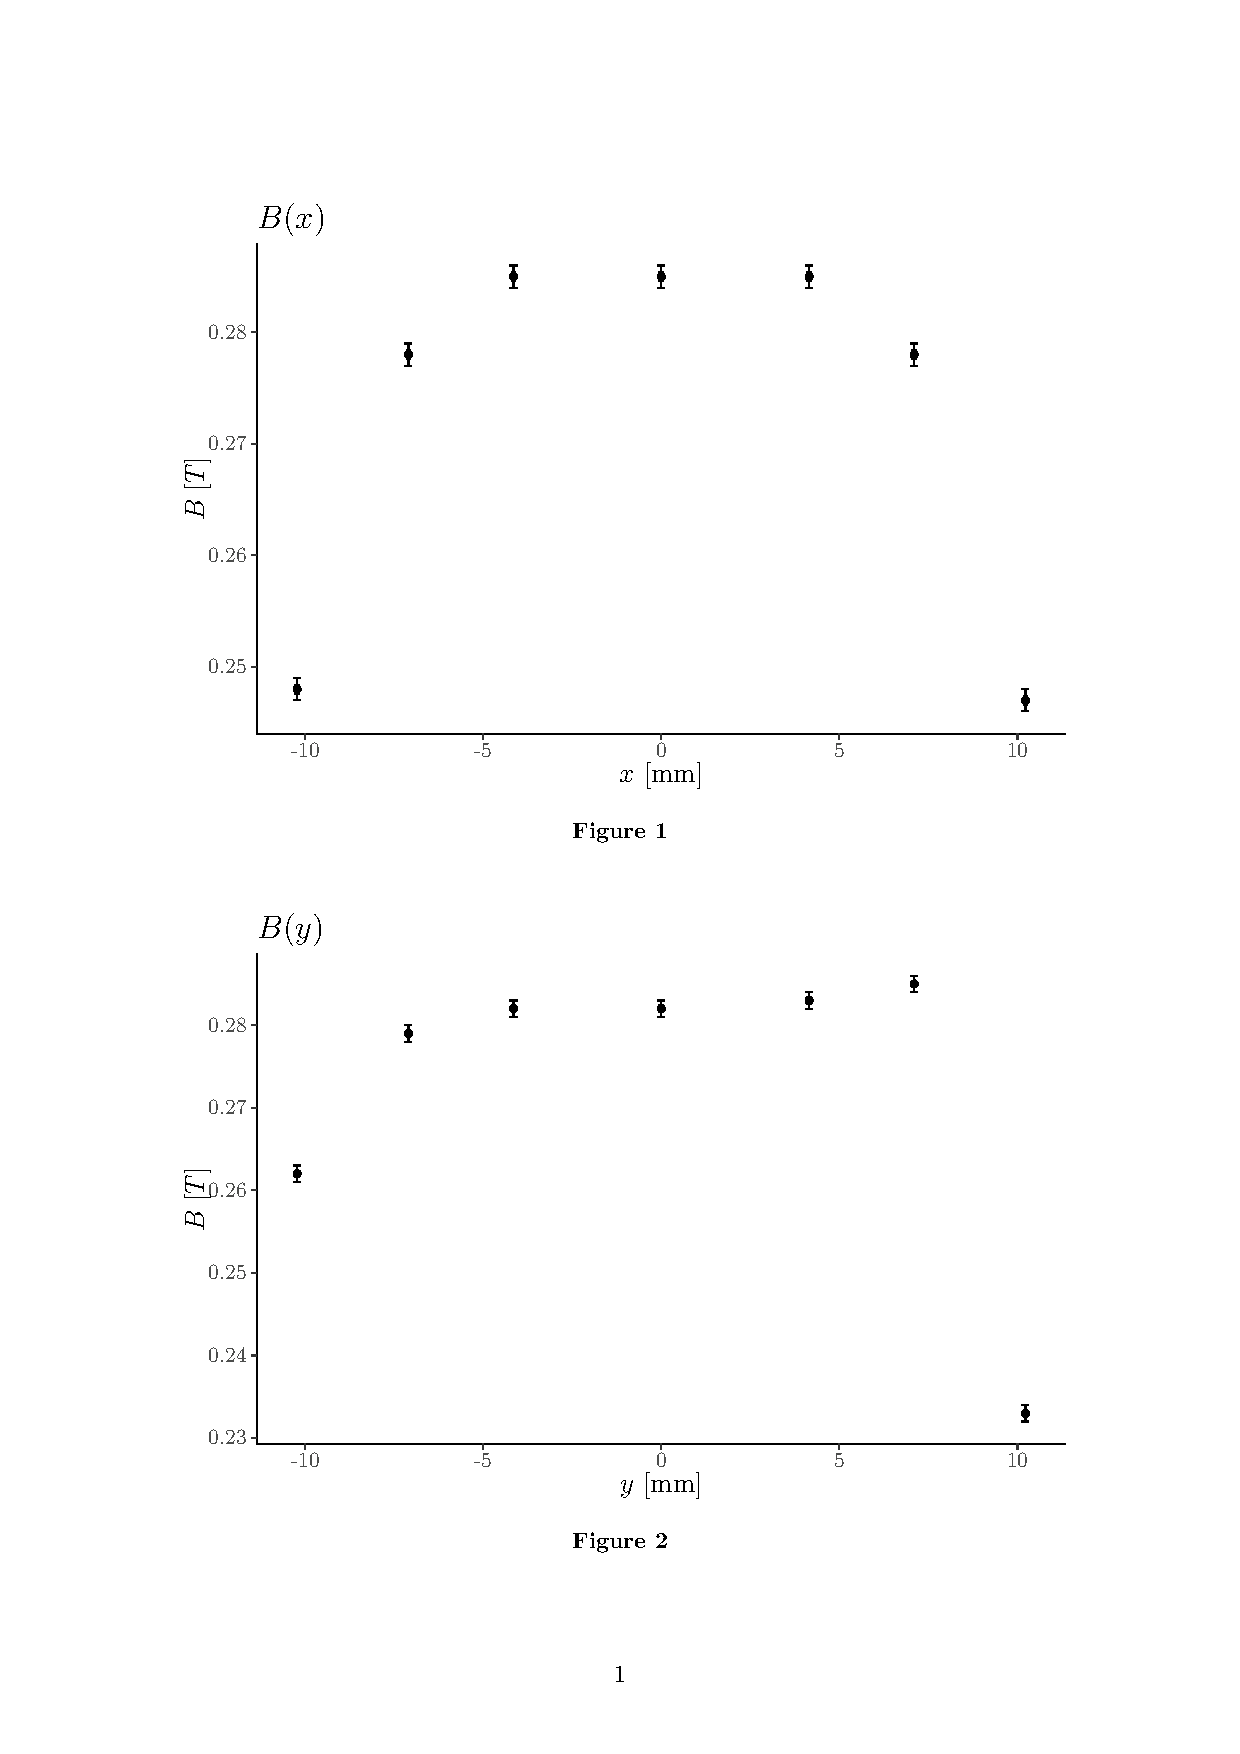
\includegraphics[trim=3cm 16.25cm 3cm 3cm, clip,height=9cm,keepaspectratio]{plots/MagneticDishomogeneity.pdf}
\end{center}
\caption{}
\label{fig:disX}
\end{figure}

\begin{table}[H]
\centering
\caption{}
\label{table:disY}
\resizebox{8cm}{!}{
\begin{tabular}{ccc}
\toprule
$I\;[A]$ & $y$ [mm] & $B\;[T]$       \\
\midrule
\rowcolor{gray!6}  4.13 $\pm$ 0.02 & -10.23 $\pm$ 0.05 & 0.262 $\pm$ 0.001\\
 & -7.10 $\pm$ 0.05  & 0.279 $\pm$ 0.001\\
\rowcolor{gray!6}   & -4.15 $\pm$ 0.05 & 0.282 $\pm$ 0.001\\
 & 0.00 $\pm$ 0.05 & 0.282 $\pm$ 0.001\\
\rowcolor{gray!6}   & 4.15 $\pm$ 0.05 & 0.283 $\pm$ 0.001\\
 & 7.10 $\pm$ 0.05 & 0.285 $\pm$ 0.001\\
\rowcolor{gray!6}   & 10.23 $\pm$ 0.05 & 0.233 $\pm$ 0.001\\
\bottomrule
\end{tabular}}
\end{table}

\begin{figure}[H]
\begin{center}
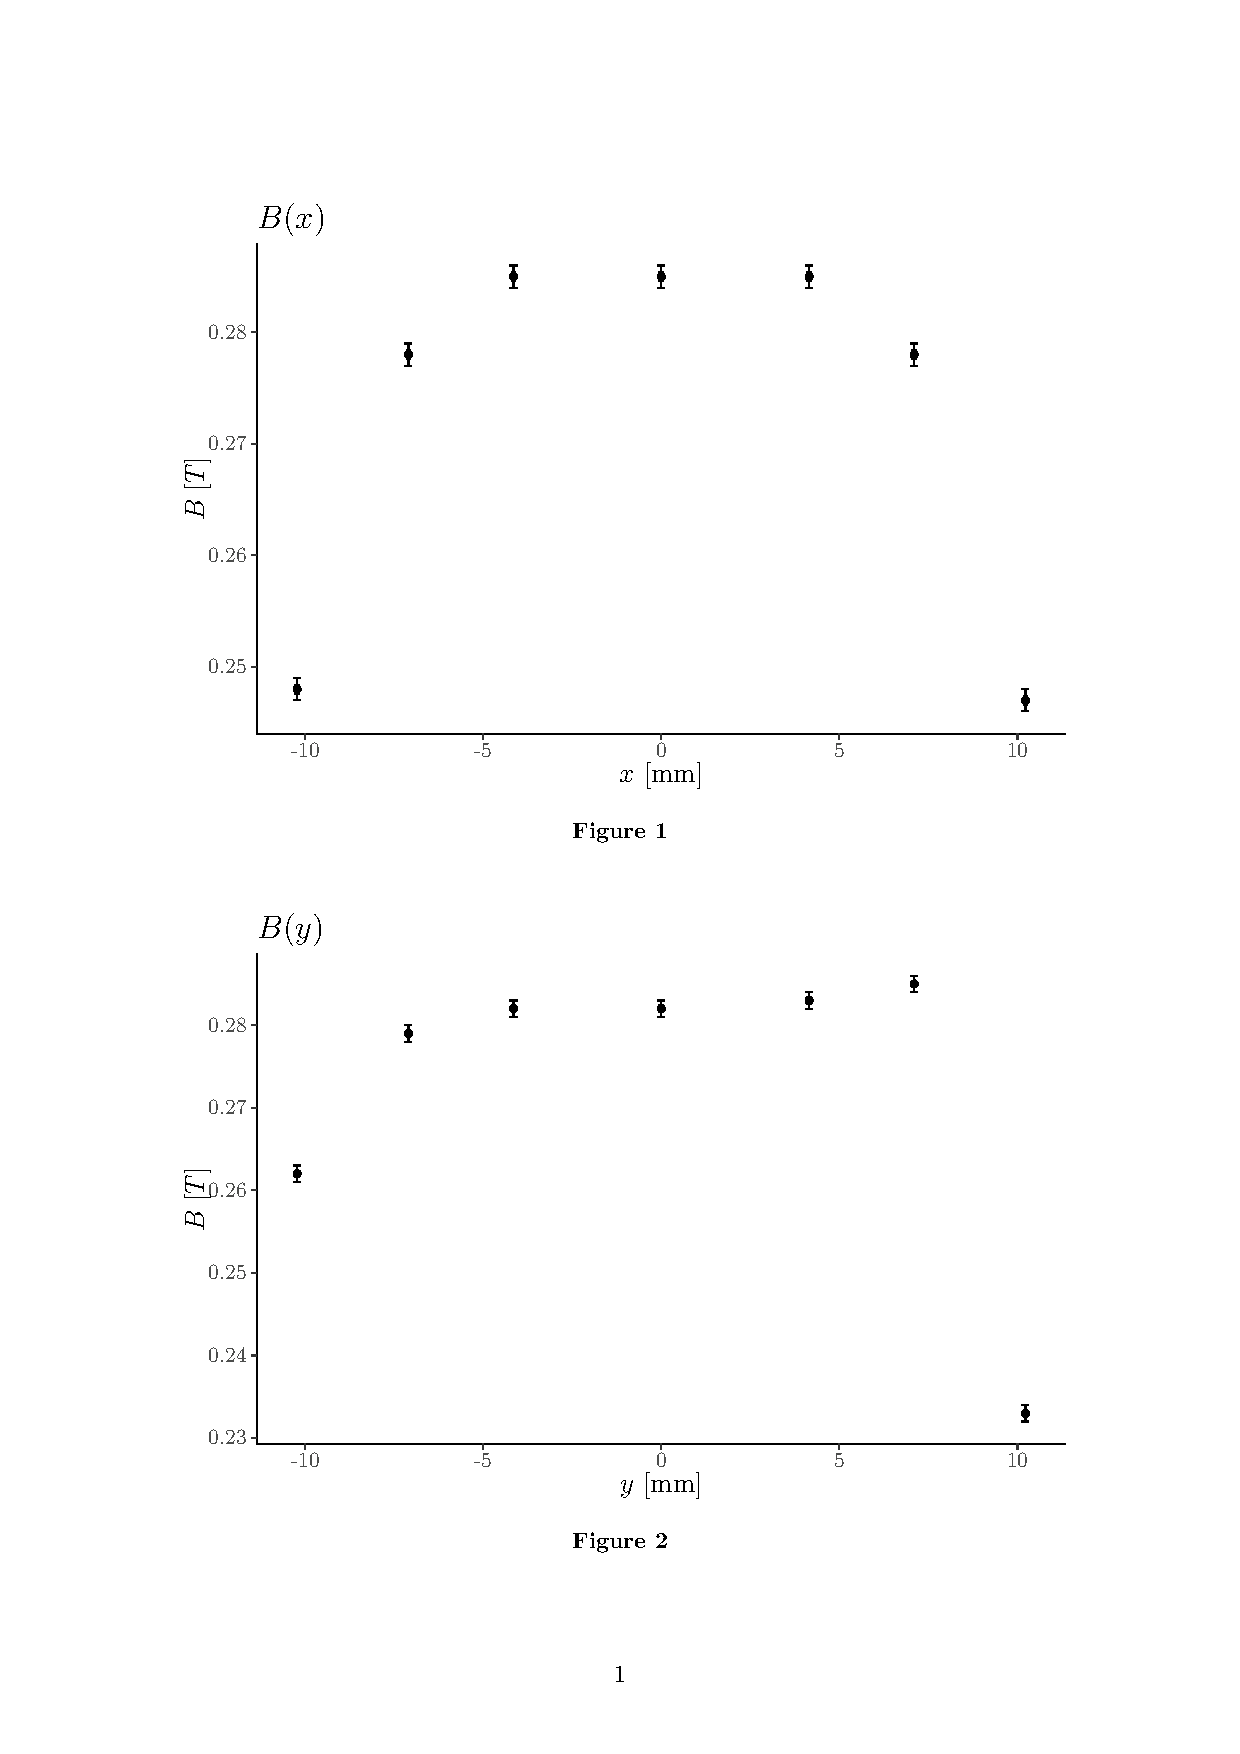
\includegraphics[trim=3cm 4cm 3cm 15cm, clip,height=7cm,keepaspectratio]{plots/MagneticDishomogeneity.pdf}
\end{center}
\caption{}
\label{fig:disY}
\end{figure}

Since the spectroscopic lamp was taller than larger, in order to evaluate the uncertainty of the magnetic field along the $x$ coordinate we have considered only the first four measures around the central position, while to evaluate it along the $y$ coordinate we have considered all the measurements and calculated the maximum semi-dispersions $\Delta_B^x=0.007 \; T$ and $\Delta_B^y=0.052 \; T$ .

Then we have computed the average of the semi-dispersions and the relative error with respect to the maximum value of $B=0.285\;T$, whose results have been reported in \hyperref[table:semi]{ Table \ref*{table:semi}}.

\begin{table}[H]
\centering
\caption{}
\label{table:semi}
\resizebox{8cm}{!}{
\begin{tabular}{cccc}
\toprule
$\Delta_B^x\;[T]$ & $\Delta_B^y\;[T]$ & $\langle \Delta_B \rangle\;[T]$ & $\Delta_{\text{rel}}$       \\
\midrule
\rowcolor{gray!6} 0.007  & 0.052  & 0.0295  & 0.1035087719\\
\bottomrule
\end{tabular}}
\end{table}

From now on the error assigned to the magnetic field will be $\Delta_B=B\Delta_{\text{rel}}$, unless the error propagation derived from the calibration curve yields a larger value. 

\clearpage

\end{document}
